% Implementation chapter of l4proj

\section{Renderer}\label{sec:renderer}
% TODO: Heartbeat
To be able to support multiple independent canvases running in a single Python kernel we need to be able to create
multiple independent renderers.
In OpenGL, only one context can be active in a given thread; in addition to this Python's global interpreter lock
prevents threads from running concurrently.
As such we decided to create a separate process for each renderer.
These render processes communicate with the Python kernel using a simple inter-process communication API built around
Python's \lstinline{multiprocessing.Queue}.

When a new canvas is created it creates a new \lstinline{SSVRenderProcessClient} which serves as the canvas' interface
to the render process.
This client starts the render process which creates a new \lstinline{SSVRenderProcessServer}.
The client and server share a receive and a transmit queue for messaging.
Renderer messages are Python tuples where the first item is a four-character command identifier, and the remaining
items are the parameters for the command.
The format of a few of the renderer commands is described below in Listing~\ref{lst:render_commands}:

\begin{lstlisting}[language=python, float, caption={The contents of a few of the different render commands.}, label=lst:render_commands]
    render = ("Rndr", target_framerate: float, stream_mode: str, encode_quality: float | None)
    stop = ("Stop", )
    update_uniform = ("UpdU", frame_buffer_uid: int | None, draw_call_uid: int | None, uniform_name: str, value: Any)
    update_vertex_buffer = ("UpdV", frame_buffer_uid: int, draw_call_uid: int, vertex_array: NDArray | None, index_array: NDArray | None, vertex_attributes: tuple[str, ...] | None)
    get_context_info = ("GtCt", query_id: int, full: bool)
\end{lstlisting}

Some commands expect a value to be returned upon completion, we refer to these as queries.
Queries have an extra item after the command identifier but before command parameters, this is the query ID. When a
query is made, the client creates a future which it stores in a dictionary.
When the query is completed the server sends back an \lstinline{ARes} command to the client containing the query ID
and the result of the query, when received, the client finds the corresponding future in its dictionary and resolves
it using the acquired query result.

The render process server creates an instance of the render which creates the OpenGL context and executes the render
commands.
The OpenGL renderer implements the \lstinline{SSVRender} interface, with the idea being that if other graphics APIs
needed to be supported, one could do so by simply implementing the \lstinline{SSVRender} interface and registering it
as a new rendering backend.
The render commands are relatively high level, so the OpenGL renderer is responsible for storing renderer objects such
as vertex buffers, textures, and render buffers, so that these can be bound to the OpenGL pipeline when needed.
The renderer also needs to perform bounds checking as needed since if it raises an uncaught exception, the render
process simply crashes without informing the user; OpenGL's error messages can also be somewhat cryptic, especially
since an error might not be raised until the next frame is rendered, as such proactive bounds checking on command
parameters can be really helpful to end users.

Since the renderer interface is command based, but we want to provide the user with an object-oriented way to interface
with the renderer, we end up mirroring the object structure used by the renderer on the canvas.
These canvas objects store a unique ID (UID) representing the corresponding renderer object and simply dispatch a
render command using the render process client, and it's UID when one of its methods are called or properties are
updated.
This allows the user to use an object-oriented interface without having to pollute the user API with renderer specific
code and keeps the renderer communication simple since we don't need to send full objects back and forth.


\section{Debugging Tools}\label{sec:debugging-tools}

A few different debugging tools were implemented to make developing shaders with \emph{pySSV} much easier.
Notably, the popular shader debugging tool: Renderdoc~\citep{karlsson_renderdoc_nodate} has been integrated.
Renderdoc is an open-source graphics API debugger, it captures all the graphics API calls in a given frame, allowing
them to be replayed and the contents of any textures/buffers/shaders to be inspected at any point in the call list.
Renderdoc includes an in-application API, which allows the application to trigger Renderdoc frame captures (among
other functions); this is necessary for \emph{pySSV} as the renderer lives in its own process which would be difficult
to attach to in Renderdoc otherwise.
The API is provided as a single C header file describing functions exported by the Renderdoc DLL\@.
Python bindings for this DLL were created using Python's \lstinline{ctypes} library.
These bindings exist as a separate Python package for modularity~\citep{mathieson_space928pyrenderdocapp_2024}. % TODO: Should this be a footnote instead of a citation? Or should it be remvoed?
A button was added to the Jupyter Widget which dispatches a render command to the renderer to trigger a frame capture
(and automatically open the Renderdoc GUI).

Additionally, public API functions are provided to view the output of the shader preprocessor and list the metadata
contained within the shader templates to help users better understand how their shaders are transformed.
Frame timing information is also provided as it can be useful in identifying where performance bottlenecks are when
rendering; the two major contributing factors to total frame time: rendering time and frame encoding time are provided
separately.


\section{Shader Preprocessor}\label{sec:shader-preprocessor}
%# DESIGN
%To reduce the amount of boilerplate shader code users need to write, we decided to implement a shader templating and
%preprocessor system this would allow the user to pick a shader template for the type of shader they want to write and
%simply write the main function and allow the preprocessor to generate the necessary boilerplate. Platform specific
%shader code such as version and extension GLSL directives should be autogenerated. Additionally, built global uniforms
%and user defined uniforms can be automatically declared by the preprocessor. Shader templates themselves range in
%complexity from barebones templates such as the pixel shader template which defines a simple vertex shader and
%includes the necessary preprocessor directives to autogenerate the needed boilerplate; to the more complex signed
%distance function template which includes a raymarching renderer and exposes an entry point to a user defined signed
%distance function. Templates can also be parameterized using template arguments.
%####
% TODO: Dynamic uniforms

With GLSL being a C-derived language, it is compatible with the C preprocessor.
The advantages of the C preprocessor: are that users are likely to be familiar with it, it can be extended by using
custom pragma directives, and a Python library for it already exists.
We used the PCPP~\citep{douglas_ned14pcpp_2024} preprocessor library as it provides many hooks to add custom behaviours
to the preprocessor, which were used substantially for this project.

When the \lstinline{canvas.shader()} method is called the shader preprocessor first runs a preprocessor to find any
\lstinline[language=GLSL]{#pragma SSV ...} directives.
The SSV directive specifies which shader template to search for; shader templates are searched for by name in the
shader template directory specified by the user first, then in the library of built-in shader templates, which are
accessed using the \lstinline{importlib.resources} library.
The preprocessor then finds all the \lstinline[language=GLSL]{#pragma SSVTemplate ...} directives in the shader
template, these are used to construct an argument parser (a Python \lstinline{argparse} instance) to parse the rest of
the arguments in the \lstinline[language=GLSL]{#pragma SSV} directive.
These parsed arguments are defined as preprocessor macros to be used by the shader template.
Finally, the shader template itself is preprocessed with the user's shader code injected into the shader template
through the use of the special \lstinline[language=GLSL]{#include "TEMPLATE_DATA"} directive which allows the shader
template author to insert the user's shader code anywhere in the template.
This process is illustrated in Fig~\ref{fig:preprocessor}.

\begin{figure}[h]
    \centering
    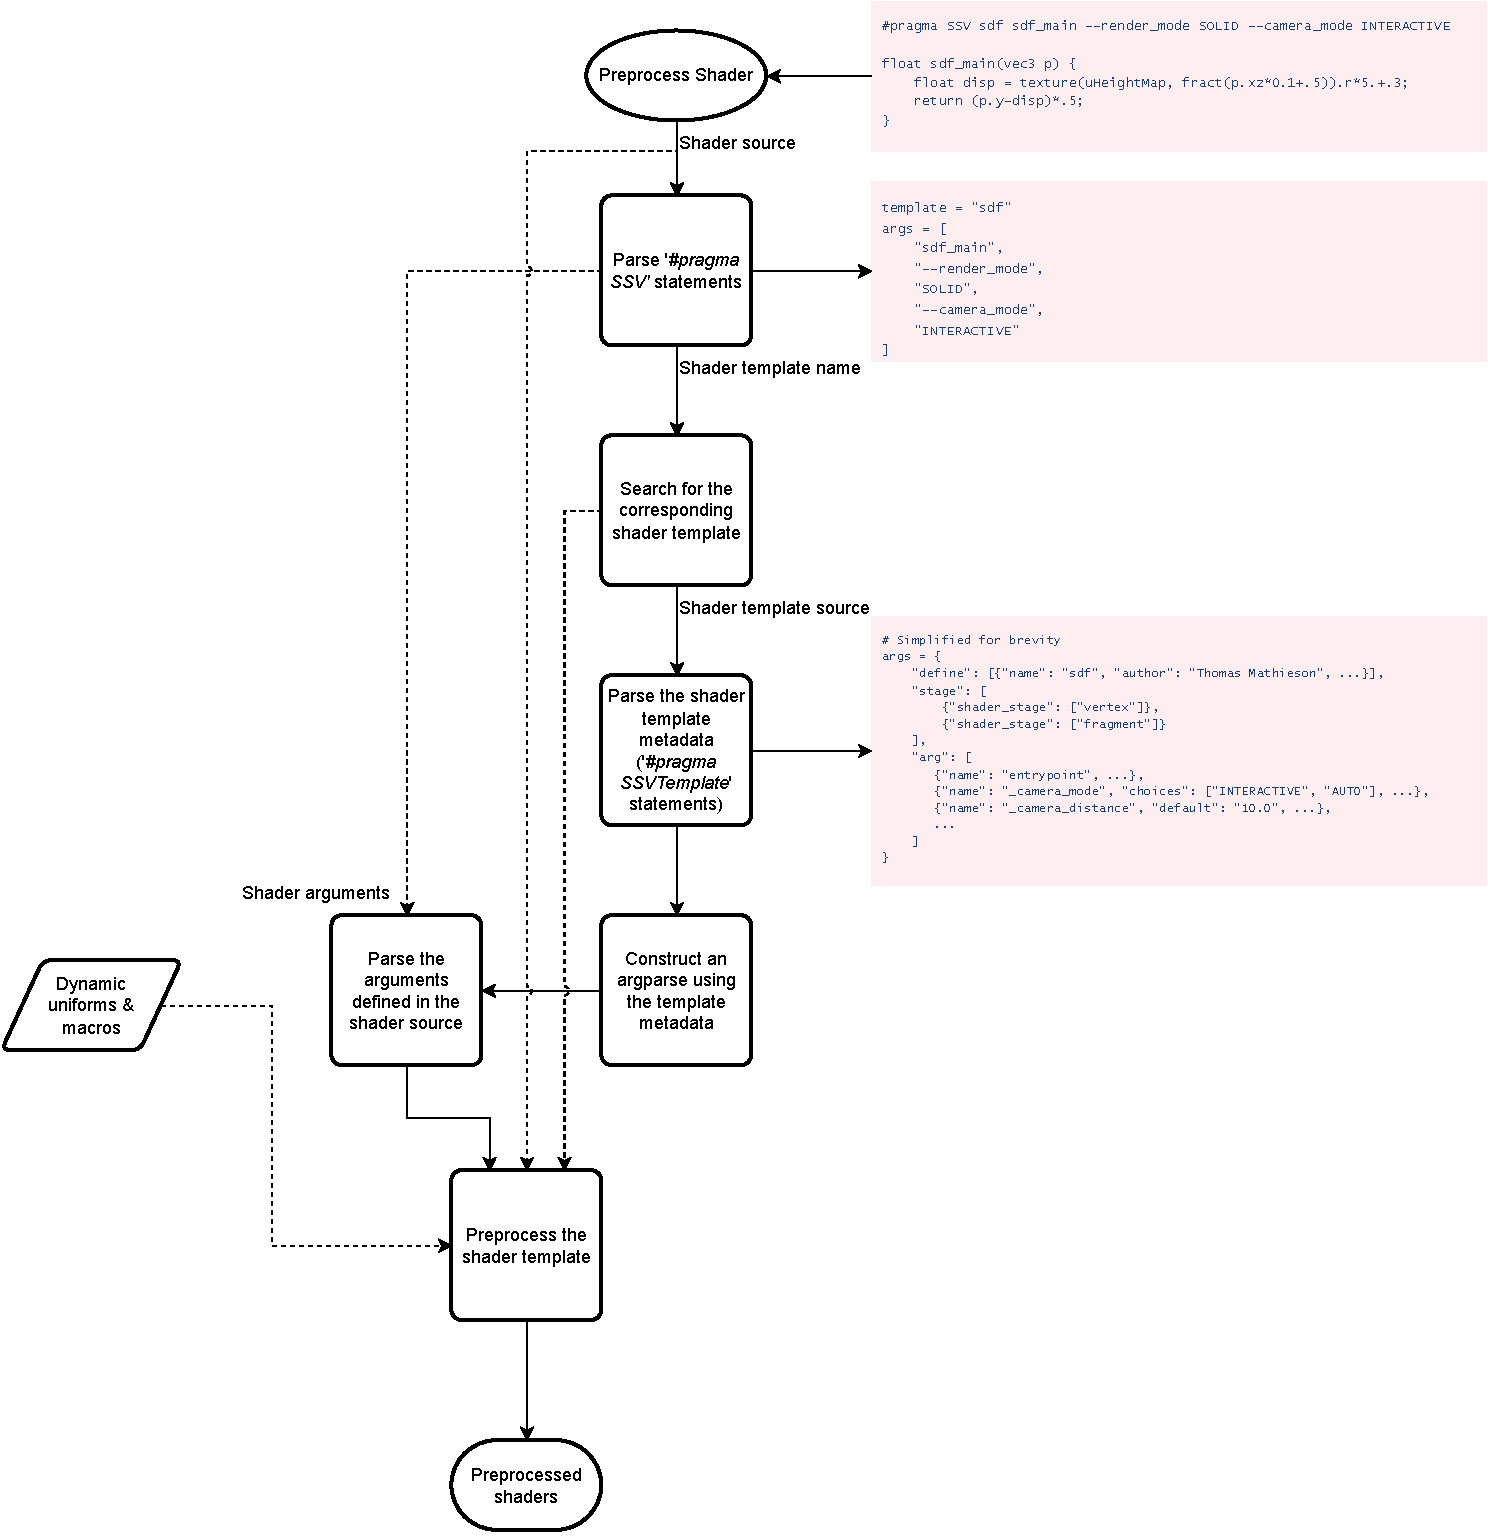
\includegraphics[width=0.8\linewidth]{images/SSV-Preprocessor}

    \caption{A flow chart describing the process of preprocessing a user shader before compilation.}

    \label{fig:preprocessor}
\end{figure}

\lstset{language=GLSL}
The shader preprocessor also defines a few special macros which expand to GLSL preprocessor directives needed by the
shader compiler such as \lstinline{#version}, \lstinline{#extension}, and \lstinline{precision}.
The \lstinline{version} directive is required in GLSL shaders and must be the very first non-whitespace/non-comment
token in the shader.
This requirement introduces some complexity, as the preprocessor by default, generates \lstinline{#line} directives,
which while very useful for debugging, can be generated before the version directive, causing a compiler error.
To solve this, we introduce a special pragma directive \lstinline{#pragma PreventLine true} which inhibits the
generation of \lstinline{#line} directives until it's disabled.
The implementation of this behaviour is a bit of a bodge due to the design of the lexer in PCPP, but it works for the
specific use case we need.
On platforms where \lstinline{#line} directives are not supported (which is the case for most non-Nvidia OpenGL
implementations) they are disabled completely by the preprocessor; to determine if line directives are supported the
\lstinline{GL_ARB_shading_language_include} extension is searched for in the OpenGL extensions list of the renderer.
\lstset{language=python}


\section{Render Widget}\label{sec:render-widget}

All Jupyter Widgets consist of three main classes: the widget view (JavaScript), the widget model (JavaScript), and the
corresponding Python widget model.
Jupyter is responsible for automatically synchronizing the fields of the JavaScript and corresponding Python models.
The widget view is implemented in three TypeScript classes, one for the main widget itself, one for the status bar,
and one for the save image settings panel.

The main view class implements the \lstinline{render()} method declared by its parent which is called by Jupyter when
the widget is created.
Inside this method, we use the standard DOM manipulation methods to create the HTML for the widget and create event
handlers for the various DOM and model events we need to listen for.
The decision to use direct DOM manipulation to render the widget instead of using a framework like React or Vue,
which could have simplified this process by allowing the use of data binding and templating, was made when the planned
complexity of the widget front end was much smaller.

The majority of the communication between the widget front end and the Python model is done using the widget's
synchronized fields.
Internally, these send JSON messages back and forth through the Jupyter server to synchronize data.
Jupyter also allows us to send custom JSON messages through this same pipe.
We use these custom messages to send event notifications for actions such as: mouse events, play/stop button presses,
heartbeat messages, etc\ldots


\section{Frame Streaming}\label{sec:frame-streaming}

Rendered frames are sent to the widget in a variety of manners depending on the codec used and the platform used.
The fallback method which works on all platforms for all streaming methods (with the notable exception of \emph{MJPEG})
is to send the data by updating a synchronized field on the widget.
This method has a few disadvantages though, the maximum data throughput is limited due to the need JSON encode and
decode all the messages.
We can save some time by using binary messages, as the Jupyter messaging protocol allows binary buffers to be attached
to JSON messages.
On locally hosted Jupyter servers, we open dedicated websocket for frame streaming.
This has the advantage of not needed to JSON-encode/decode stream data before it's sent;
it also provides marginally better latency as the data doesn't have to wait for the Jupyter server's asynchronous
dispatcher.
Additionally, if the frame data becomes backed up on the client side (if for instance frames can't be decoded fast
enough), control messages from the Jupyter UI won't be delayed.
On platforms such as Google Colab, the use of a dedicated websocket server isn't possible due to the platform's
proxying limitations as described in \citet{adaickalavan_websocket_nodate}.

% TODO: Maybe we should dedicate a section of the Evaluation to provide data proving the statements here
For the \emph{PNG} and \emph{JPG} streaming modes, the frames are streamed directly into an HTML
\lstinline[language=HTML]{<img>} element.
We do this by encoding the streamed frame as a base64 encoded data URL in Python and copying it into the image element's
\lstinline{src}; this has the advantage that the web browser decodes the image natively, as opposed to having to decode
the image from a binary buffer in JavaScript, which would be much slower. % TODO: data to back this up?
Since the stream data is already encoded as a string, it's faster to send it in a string field when using synchronized
fields, avoiding the need to use a JavaScript \lstinline[language=JS]{TextDecoder}. % TODO: data to back this up?
These formats perform well on locally hosted Jupyter instances, where network bandwidth is a non-issue, \emph{JPG} in
particular is very fast to encode/decode. \emph{PNG} is the only streaming format we support which can transport
lossless images. % TODO: Move this sentence to design?

In an effort to reduce network bandwidth use when streaming frames, we implemented support for a few video codecs; these
have the advantage of reducing network utilization, but take longer to encode/decode. % TODO: data
As it turns out Google Colab batches Jupyter messages together, which means that even if we reduce the streaming
data rate by using a video codec, the effective frame rate/latency is still limited by the rate Google Colab will send
Jupyter messages.
We chose to support the \emph{H.264}, \emph{VP8}, and \emph{VP9} video codecs as these are relatively fast to encode,
supported by our encoder (FFmpeg~\citep{ffmpeg_developers_ffmpeg_2024}), and the decoder (the
WebCodecs~API~\citep{adenot_webcodecs_2024}).
Using the WebCodecs API allows the web browser to offload video decoding from JavaScript to native code (which may be
hardware accelerated).
The disadvantage of WebCodecs is that it has fairly limited (and platform dependent) support for video codecs; the
Firefox browser is entirely unsupported as of writing, the full list of supported codecs on a given browser can be
tested here \footnote{https://cconcolato.github.io/media-mime-support/}.
In future, support for Firefox and other video codecs could be added by including a JavaScript/WebAssembly polyfill for
the WebCodecs API\@.
Decoded video frames are blitted into an HTML \lstinline[language=HTML]{<canvas>} element.
Video encoding is handled by FFmpeg, specifically, we use the pyAV~\citep{pyav_developpers_pyav_2024} bindings for the
FFmpeg libavformat and libavcodec libraries.
Currently, video encoding happens entirely on the CPU due to the extra complexity involved in getting GPU accelerated
video encoding to work on all platforms; this is something that could be improved in the future.

The \emph{MJPEG} streaming mode is handled differently from the other streaming formats.
This format is simply a stream of \emph{JPG} images sent as one indefinite multipart HTTP request.
To implement this, we host a simple HTTP server, and as such this format only supports local Jupyter instances, which
responds to \lstinline{GET} requests with a \lstinline{multipart/x-mixed-replace} MIME type which instructs the browser
that the response will consist of many separate HTTP responses.
The HTML image element is simply pointed at the local HTTP server decodes frames automatically as they arrive.
This has the advantage that the frame data never needs to be touched by the JavaScript which can be quite slow, as
such this method has the lowest latency. % TODO: data


\section{Quality of Life Features}\label{sec:quality-of-life-features}

A few extra features are provided in the library to solve common problems and reduce boilerplate code.
They are described in detail in this section.


\subsection{GUI Library}\label{subsec:gui-library}

To allow users to interact with their shaders a GUI library is provided which includes a basic automatic layout system
and a number of built-in controls.
The API is design to emulate classic immediate-mode GUI libraries, but due to the implementation of the layout system,
elements aren't actually drawn until all GUI elements have been created.

% TODO: Write this up in plain English...
% General GUI update/layout process
\begin{lstlisting}[language=none,label={lst:temp-gui-update}]
    # TODO: Write this out nicely, maybe as a flow chart?
    Mouse move, Click, Keyboard event
    \/
    Redraw GUI():
        Clear caches
        Draw main GUI layout container
        \-> Draw Layout Group()

    Draw Layout Group():
        Apply padding as needed
        Call the pre-layout callbacks on all children
        Compute child element spacing  # (elements may need to be squeezed, different elements take up different amounts of space)
        for el in children:
            Compute target rectangle
            Draw child
            \-> Draw Layout Container() or Draw GUI Element()

    Draw GUI Element():
        # This function is different for each GUI element, but they generally involve the following:
        Determine shader mode  # (which shader features are needed for GUI element; GUI elements which use the same shader features are batched into the same draw call)
        Get vertex buffer  # (Vertex buffers are cached and aren't resized unless needed to reduce pressure on the memory allocator)
        Generate vertices for this GUI element
        # For GUI elements which return a result (sliders, buttons, etc...):
            Update result variable
\end{lstlisting}

% Layout engine details
\begin{lstlisting}[language=none,label={lst:temp-gui-layout}]
    class LayoutGroup:
        vertical: bool  # The direction child elements should flow in
        squeeze: bool   # Whether child elements should attempt to be squeezed to fit in the container as opposed to overflowing
        pad: bool       # Whether this container should be padded (using the global padding value)
        children: list[GUIElement]  # List of child elements, which can include other layout groups

    class GUIElement:
        expand: bool    # Whether this element can be squeezed or expanded in the layout direction
        layout: bool    # Whether this element should participate in automatic layout
        overlay_last: bool  # Whether this element should copy the last element's layout, enabling this also has the effect of disabling 'layout'
        width: int      # The desired width of the element, may be squeezed to fit the container
        height: int     # The desired height of the element, may be squeezed to fit the container
\end{lstlisting}
The layout engine's job is to divide a given rectangle of the screen that the layout group occupies into separate
rectangles for each child element.
A layout group flows either horizontally or vertically (at the moment either left-to-right or top-to-bottom); when
flowing top-to-bottom, elements with a fixed height (ie: \lstinline{expand} is \lstinline{False}) are placed one after
the other with some padding between them.
If an element has the \lstinline{expand} field set to \lstinline{True}, the layout engine attempts share all the
remaining space (that is the group height minus the sum of the heights of the fixed height elements) evenly; if the
group's \lstinline{squeeze} property is \lstinline{True} then child elements with \lstinline{expand} enabled will be
squeezed smaller than their \lstinline{height} to fit, otherwise the minimum height of the child element is clamped to
its \lstinline{height} property and elements which don't fit inside the layout group are clipped.
In this case the element's width is the minimum of layout group's width and the element's width.
For layout groups with a horizontal flow-direction, this process is the same, swapping width for height.
The \lstinline{layout} property determines whether an element in a layout group participates in automatic layout or not,
when disabled, the element is ignored while calculating the layout rectangles, it's height/width are not taken into
account, the element is still drawn in the correct order, but is given the full rectangle of the layout group and
expected to place itself sensibly.
The \lstinline{overlay_last} property acts similarly to \lstinline{layout = False} when set, with the exception being
that the rectangle passed to element's draw function is the rectangle of the last element to be laid out.
This is useful for controls composed of multiple elements such as the checkbox, where the checkmark should overlay the
checkbox when checked.

% Input handling

% Batching
    % Creating/destroying OpenGL buffers is slow
    % Having many small draw calls is much slower than a few larger ones
    % UI elements which use the same shader can be batched into a single draw call by merging vertex buffers
        % To support this, shader parameters which would have otherwise been uniforms, become custom vertex attributes
    % We maintain a dictionary cache of vertex buffers and corresponding NumPy arrays (so that the updated vertices
      % can be copied to the destination vertex buffer all at once), where the key of the dictionary is an int of bit
      % flags representing the enabled shader features
        % We avoid resizing the array/vertex buffer so long as the requested number of vertices fit to avoid
          % reallocations. At the end of the draw, excess vertex array/buffer capacity is trimmed; hence if no gui
          % elements are created or destroyed between two frames, no buffers need reallocating.

% GUI shader
    % Use of the preprocessor to strip code
    % Text rendering
        % Brief on SDF & multi-channel SDF fonts (might belong in the design section?)
        % Font asset generation using msdf-gen
        % Anglecode font parser
        % Text rendering
            % Hinting
            % Text effects
                % Shadow
                % Font weight
                % Italic
    % Rounded corners
    % Outlines

% TODO: Should it be a flow chart instead?
\begin{algorithm}
    \DontPrintSemicolon
    \Begin{
        $padding \longleftarrow []$\;
        \ForAll{$children$}
        
        \EndFor
    }

    \caption{This algorithm describes the process by which the GUI is automatically layed out and drawn.}
    \label{alg:gui-draw}
\end{algorithm}

\subsection{Camera}\label{subsec:camera}

% TODO: I don't have much to say about this, but might be worth mentioning

\subsection{Shader Library}\label{subsec:shader-library}

% TODO: There's not too much to say about this; it's mostly a library of standard functions, some written by myself, others sourced from the internet.
% I could briefly discuss the different shader templates here, but they're also already described in the documention...

\section{Packaging}\label{sec:packaging}

While the source code to this project is published on GitHub, to allow for easy installation by users \emph{pySSV} is
published on PyPi\footnote{https://pypi.org/project/pySSV/} and npm\footnote{https://www.npmjs.com/package/py-ssv}.
Because the project includes a Python backend and a TypeScript frontend, we need to publish it on two different package
repositories.
npm doesn't support Python packages, and Jupyter clients (such as JupyterLab, VSCode, Google Colab, etc\ldots) rely on
CDNs such as jsDelivr and unpkg which automatically host all packages published on npm.
For stability, JupyterLab uses its own package manager \lstinline{jlpm} which is a pinned version of the popular
package manager \lstinline{yarn}.
The frontend package can only be built using jlpm due to version constraints, but to publish on npm requires
an up-to-date yarn lock file.
This results in needing to build the project after installing the dependencies with jlpm, and then reinstalling the
dependencies using yarn before publishing; the full instructions for this are in the \lstinline{RELEASING.md} file in
the source code repository.
Managing dependencies for complex projects can be difficult, and for now this solution works, but in future we should
aim to make everything build with yarn, or wait for jlpm to be updated. % TODO: How do other packages solve this problem?

